% Options for packages loaded elsewhere
\PassOptionsToPackage{unicode}{hyperref}
\PassOptionsToPackage{hyphens}{url}
%
\documentclass[
  17pt,
  a4paper]{extarticle}
\title{Analysis 1B --- Tutorial 5}
\author{Christian Jones: University of Bath}
\date{March 2023}

\usepackage{amsmath,amssymb}
\usepackage{lmodern}
\usepackage{iftex}
\ifPDFTeX
  \usepackage[T1]{fontenc}
  \usepackage[utf8]{inputenc}
  \usepackage{textcomp} % provide euro and other symbols
\else % if luatex or xetex
  \usepackage{unicode-math}
  \defaultfontfeatures{Scale=MatchLowercase}
  \defaultfontfeatures[\rmfamily]{Ligatures=TeX,Scale=1}
\fi
% Use upquote if available, for straight quotes in verbatim environments
\IfFileExists{upquote.sty}{\usepackage{upquote}}{}
\IfFileExists{microtype.sty}{% use microtype if available
  \usepackage[]{microtype}
  \UseMicrotypeSet[protrusion]{basicmath} % disable protrusion for tt fonts
}{}
\makeatletter
\@ifundefined{KOMAClassName}{% if non-KOMA class
  \IfFileExists{parskip.sty}{%
    \usepackage{parskip}
  }{% else
    \setlength{\parindent}{0pt}
    \setlength{\parskip}{6pt plus 2pt minus 1pt}}
}{% if KOMA class
  \KOMAoptions{parskip=half}}
\makeatother
\usepackage{xcolor}
\IfFileExists{xurl.sty}{\usepackage{xurl}}{} % add URL line breaks if available
\IfFileExists{bookmark.sty}{\usepackage{bookmark}}{\usepackage{hyperref}}
\hypersetup{
  pdftitle={Analysis 1B --- Tutorial 5},
  pdfauthor={Christian Jones: University of Bath},
  hidelinks,
  pdfcreator={LaTeX via pandoc}}
\urlstyle{same} % disable monospaced font for URLs
\usepackage[margin=2.5cm]{geometry}
\usepackage{longtable,booktabs,array}
\usepackage{calc} % for calculating minipage widths
% Correct order of tables after \paragraph or \subparagraph
\usepackage{etoolbox}
\makeatletter
\patchcmd\longtable{\par}{\if@noskipsec\mbox{}\fi\par}{}{}
\makeatother
% Allow footnotes in longtable head/foot
\IfFileExists{footnotehyper.sty}{\usepackage{footnotehyper}}{\usepackage{footnote}}
\makesavenoteenv{longtable}
\usepackage{graphicx}
\makeatletter
\def\maxwidth{\ifdim\Gin@nat@width>\linewidth\linewidth\else\Gin@nat@width\fi}
\def\maxheight{\ifdim\Gin@nat@height>\textheight\textheight\else\Gin@nat@height\fi}
\makeatother
% Scale images if necessary, so that they will not overflow the page
% margins by default, and it is still possible to overwrite the defaults
% using explicit options in \includegraphics[width, height, ...]{}
\setkeys{Gin}{width=\maxwidth,height=\maxheight,keepaspectratio}
% Set default figure placement to htbp
\makeatletter
\def\fps@figure{htbp}
\makeatother
\setlength{\emergencystretch}{3em} % prevent overfull lines
\providecommand{\tightlist}{%
  \setlength{\itemsep}{0pt}\setlength{\parskip}{0pt}}
\setcounter{secnumdepth}{5}
\newcommand{\BOO}{BOO}
\usepackage {hyperref}
\hypersetup {colorlinks = true, linkcolor = blue, urlcolor = blue}
\usepackage{float}
\ifLuaTeX
  \usepackage{selnolig}  % disable illegal ligatures
\fi

\usepackage{amsthm}
\theoremstyle{plain}
\newtheorem*{theorem*}{Theorem}\newtheorem{theorem}{Theorem}[section]
\theoremstyle{definition}
\newtheorem*{definition*}{Definition}\newtheorem{definition}{Definition}[section]
\theoremstyle{plain}
\newtheorem*{proposition*}{Proposition}\newtheorem{proposition}[theorem]{Proposition}
\newtheorem*{Definitions*}{Definitions}\newtheorem{Definitions}[definition]{Definitions}
\theoremstyle{plain}
\newtheorem*{lemma*}{Lemma}\newtheorem{lemma}{Lemma}[section]
\theoremstyle{plain}
\newtheorem*{corollary*}{Corollary}\newtheorem{corollary}{Corollary}[section]
\theoremstyle{plain}
\newtheorem*{conjecture*}{Conjecture}\newtheorem{conjecture}{Conjecture}[section]
\theoremstyle{definition}
\newtheorem*{example*}{Example}\newtheorem{example}{Example}[section]
\theoremstyle{definition}
\newtheorem*{exercise*}{Exercise}\newtheorem{exercise}{Exercise}[section]
\newtheorem*{Thought*}{Thought}\newtheorem{Thought}{Thought}[section]
\theoremstyle{remark}
\newtheorem*{remark*}{Remark}
\newtheorem*{solution*}{Solution}
\newtheorem*{Example*}{Example}
\theoremstyle{remark}
\newtheorem*{Proof*}{Proof}
\newtheorem*{Examples*}{Examples}
\let\BeginKnitrBlock\begin \let\EndKnitrBlock\end


%\usepackage[english,shorthands=off]{babel}
\usepackage{etoolbox}
\usepackage{spverbatim}
\makeatletter
\@ifpackageloaded{float}{}{\usepackage{float}}
\@ifpackageloaded{adjustbox}{}{\usepackage[Export]{adjustbox}}
\makeatother
\floatplacement{figure}{H}
\newcommand{\scalefactor}{1.7}
\adjustboxset*{min width=\scalefactor\width,max width=\linewidth}
\renewcommand{\familydefault}{phv}
\fontfamily{phv}\selectfont
\renewcommand{\em}{\bf}\renewcommand{\textit}{\textbf}\renewcommand{\emph}{\textbf}\renewcommand{\it}{\bf}\renewcommand{\itshape}{\bf}
\setlength{\parindent}{0.0pt}
\setlength{\parskip}{1.0\baselineskip}
\renewcommand{\baselinestretch}{1.5}\selectfont
\setlength{\mathsurround}{0.2em}
\setlength{\arraycolsep}{0.5cm}\renewcommand{\arraystretch}{1.5}
\addtolength{\jot}{\baselineskip}
\renewcommand{\;}{\,}
\sloppy
\allowdisplaybreaks
\usepackage{amsthm}
\newtheoremstyle{plain}{20pt}{3pt}{}{}{\bfseries}{.\newline\nobreak}{1.0em\nobreak}{}
\newtheoremstyle{definition}{20pt}{3pt}{}{}{\bfseries}{.\newline\nobreak}{1.0em\nobreak}{}
\newtheoremstyle{remark}{20pt}{3pt}{}{}{\bfseries}{.\newline\nobreak}{1.0em\nobreak}{}
\csundef{Proof}
\csundef{endProof}
\newenvironment{Proof}
  {\noindent{\bf Proof.}\hspace*{1em}}% Begin
  {\qed\par}% End
%% When redefining an environment it is vital that it has 
%% the same number of arguments as the original
\renewenvironment{proof}[1][\proofname]
  {\trivlist\item\relax\noindent{\bf {#1}.}\hspace*{1em}}% Begin
  {\qed\endtrivlist}% End

\begin{document}
\maketitle

{
\setcounter{tocdepth}{2}
\tableofcontents
}
\newpage
\pagenumbering{arabic}

\hypertarget{introduction}{%
\section*{Introduction}\label{introduction}}
\addcontentsline{toc}{section}{Introduction}

Here is the material to accompany the 5th Analysis 1B Tutorial on the 6th March. Alternative formats can be downloaded by clicking the download icon at the top of the page. Please send any comments or corrections to \href{mailto:caj50@bath.ac.uk}{Christian Jones (caj50)}. To return to the homepage, click \href{http://caj50.github.io/tutoring.html}{here}.

\hypertarget{lecture-recap}{%
\section{Lecture Recap}\label{lecture-recap}}

After what was mainly revision last week, we're moving onto some new stuff again! It turns out there's still a bit we can say about continuity, especially on compact intervals.

\hypertarget{inverse-functions}{%
\subsection{Inverse Functions}\label{inverse-functions}}

A particularly useful class of functions we may be interested in are known as invertible. These functions \(f: A \to B\) provide a way of moving between sets \(A\) and \(B\) (and back again) without losing any information about \(A\) and \(B\). Before we talk about them in more detail, it's worth recalling some definitions:

\BeginKnitrBlock{definition}[Injectivity, Surjectivity and Bijectivity]
{\label{def:def1} }Let \(f: A \to B\) be a function.

\begin{itemize}
\tightlist
\item
  If \(\forall x, y \in B\) with \(x \neq y\), \(f(x) = f(y) \implies x = y\), then \(f\) is said to be injective.
\item
  If \(\forall y \in B\), \(\exists x \in A\) such that \(f(x) = y\), then \(f\) is surjective.
\item
  If \(f\) is both injective and surjective, then it is called bijective.
\end{itemize}
\EndKnitrBlock{definition}

In words, bijectivity means that for a function \(f:A \to B\), every element in the codomain \(B\) is mapped to by a unique element in the domain \(A\). These bijective functions are said to be invertible, that is, there exists an inverse function \(f^{-1}: B \to A\) such that \(f^{-1} \circ f\) and \(f \circ f^{-1}\) produce the identity maps on \(A\) and \(B\) respectively.

Now that we have these definitions, we can say something about the continuity of inverse functions:

\BeginKnitrBlock{theorem}
{\label{thm:thm1} }Let \(I \subseteq \mathbb{R}\) be a non-empty\footnote{This is so we can talk about surjectivity.} interval, and let \(f: I \to \mathbb{R}\) be continuous on \(I\). Assume that \(f\) is strictly increasing\footnote{In other words, for all \(x,y \in I\) with \(x < y,\) \(f(x) < f(y)\).} (or strictly decreasing) on \(I\). Then:

\begin{itemize}
\tightlist
\item
  \(J:=f(I)\) is an interval,
\item
  \(f : I \to J\) is bijective, and
\item
  \(f^{-1}: J \to I\) is continuous on \(J\).
\end{itemize}
\EndKnitrBlock{theorem}

You've seen an example of this theorem in action in the lectures. This is repeated below, as we're going to use it to prove a powerful result regarding sequences.

\BeginKnitrBlock{example}
{\label{exm:ex1} }Consider the exponential function \(\exp:\mathbb{R} \to \mathbb{R}\) defined by \[\exp(x)  = \sum_{n = 0}^{\infty} \frac{x^n}{n!} = \mathrm{e}^x.\] Firstly, note that \(\mathbb{R}\) is a non-empty interval. Now, using some results from Semester 1, we know that

\begin{itemize}
\tightlist
\item
  \(\exp\) is continuous and strictly increasing on \(\mathbb{R}\), and
\item
  \(\exp(\mathbb{R}) = (0,\infty)\).
\end{itemize}

Therefore, \(\exp\) satisfies the hypotheses of the above theorem, and so \(\exp: \mathbb{R} \to (0, \infty)\) is a bijection, with continuous inverse. This inverse function is the well-known \emph{natural logarithm} \(\ln: (0,\infty) \to \mathbb{R},\) where \(x = \ln(y) \iff y = \exp(x).\)

We can plot the graphs of \(y = \exp(x)\) (in red), and \(y = \ln(x)\) (in blue) to visually see that Theorem \ref{thm:thm1} works. Also note that to plot the graph of an inverse function, we only need to reflect the graph of the original function through the line \(y=x\) (dashed green line).

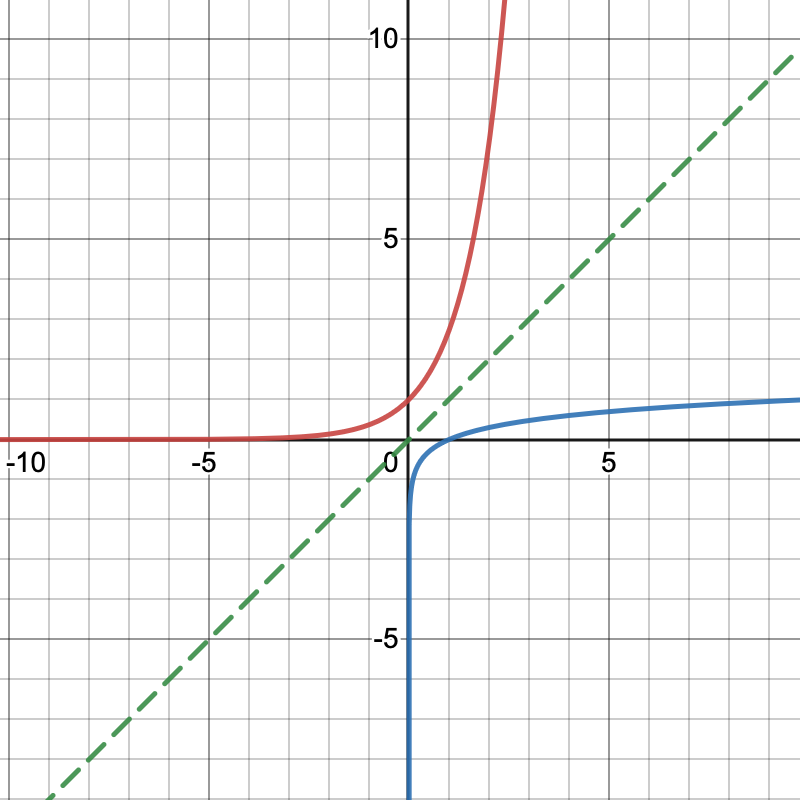
\includegraphics[width=0.3\textwidth,height=\textheight]{./explog.png}
\EndKnitrBlock{example}

Now that we have this example, we can easily calculate another large class of sequence limits:
\BeginKnitrBlock{proposition}
{\label{prp:prop1} }Let \((a_n)_n\) and \((b_n)_n\) be real sequences such that \(\lim_{n\to\infty}a_n = a\) and \(\lim_{n\to\infty}b_n = b\). If \(a_n^{b_n} \in \mathbb{R}\;\; \forall n \in \mathbb{N}\), and \(a>0\), then \[\lim_{n \to \infty} a_n^{b_n} = \left(\lim_{n\to\infty} a_n\right)^{\lim_{n\to\infty}b_n}.\]
\EndKnitrBlock{proposition}

\textbf{Proof}

\BeginKnitrBlock{proof}
Since \(\lim_{n \to \infty}a_n = a > 0\), then \(\exists N\in\mathbb{N}\) such that \(\forall n \geq N\), \[\lvert a_n - a \rvert < \frac{a}{2} \Longleftrightarrow \frac{a}{2} < a_n < \frac{3a}{2}.\] In particular, \(a_n > 0\) for all \(n \geq N\).

Now, for \(n \geq N\),
\begin{align*}
a_n^{b_n} &= \exp\left(\ln\left(a_n^{b_n}\right)\right)\;\;\text{(as $a_n > 0$)},\\
&= \exp\left(b_n\ln\left(a_n\right)\right)\;\;\text{(properties of $\ln$)}.
\end{align*}
So as \(n \to \infty\), we have that as both \(\exp\) and \(\ln\) are continuous (Example \ref{exm:ex1}),
\begin{align*}
a_n^{b_n} &\to \exp\left(b\ln(a)\right)\\
&= \exp\left(\ln\left(a^b\right)\right),\\
&= a^b.
\end{align*}
\EndKnitrBlock{proof}

\hypertarget{weierstrass-extremal-theorem}{%
\subsection{Weierstrass Extremal Theorem}\label{weierstrass-extremal-theorem}}

Much like the Intermediate Value Theorem, we can obtain some special continuity results when our functions are defined on compact (i.e.~closed and bounded) intervals. One of the main results from this week is stated below:

\BeginKnitrBlock{theorem}[Weierstrass Extremal Theorem (WET)]
{\label{thm:thm2} }Let \(a,b \in \mathbb{R}\) with \(a<b\), and let\footnote{Recall that \(C^{0}([a,b])\) is the set of continuous functions mapping from the set \([a,b]\).} \(f \in C^{0}([a,b])\). Then:

\begin{enumerate}
\def\labelenumi{\arabic{enumi}.}
\item
  \(f\) is bounded: \[\exists M > 0 \;\;\text{s.t.}\;\; \lvert f(x) \rvert \leq M\;\;\forall x \in [a,b].\]
\item
  \(f\) attains its bounds: \[\exists p,q \in [a,b] \;\; \text{s.t}\;\; \forall x \in [a,b], f(q) \leq f(x) \leq f(p).\]
\end{enumerate}
\EndKnitrBlock{theorem}

This last point states that if \(f \in C^{0}([a,b])\), \[\sup_{x \in [a,b]}f(x) = \max_{x\in[a,b]}f(x)\;\;\text{and}\;\;\inf_{x \in [a,b]}f(x) = \min_{x\in[a,b]}f(x).\] So in fact, what this theorem tells us is that for a function defined on a compact interval, we have some control on its growth, and we know that the function has a maximum and minimum value! This can be seen pictorally in Figure \ref{fig:wet}.

\begin{figure}
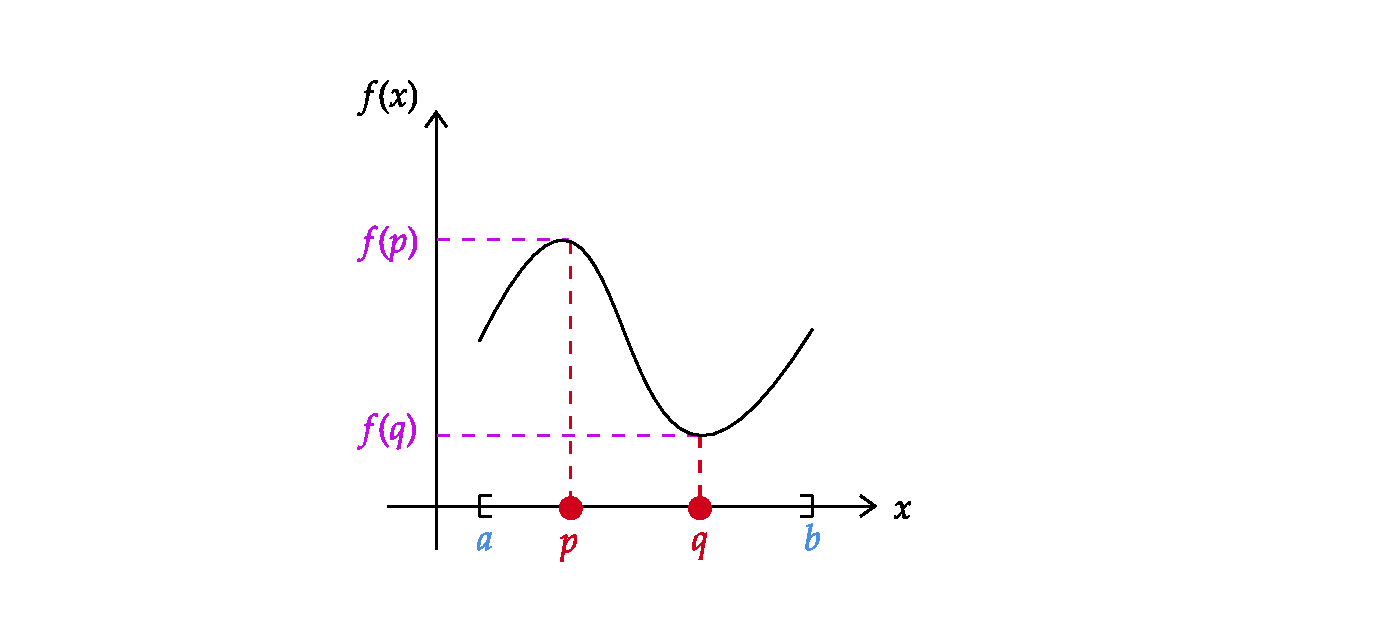
\includegraphics[width=\Width,height=\Height]{WET} \caption{This function $f$ is continuous on $[a,b]$, so by the Weierstrass Extremal Theorem, $f$ is bounded on $[a,b]$. Also, we see that there exist points $p$ and $q$ in the domain at which $f$ achieves its maximum and minimum values.}\label{fig:wet}
\end{figure}

\hypertarget{hints}{%
\section{Hints}\label{hints}}

As per usual, here's where you'll find the problem sheet hints!

\begin{enumerate}
\def\labelenumi{\arabic{enumi})}
\item
  This one is largely similar to the one that was covered in tutorials --- you just need to be a bit more careful when verifying the hypothesis of the theorem involving inverse functions. When proving bijectivity, you can use results from tutorial question 1 to help too!
\item
  \begin{enumerate}
  \def\labelenumii{\roman{enumii})}
  \tightlist
  \item
    The question you're trying to answer here is does \(\max_{[a,x]}f(x)\) exist?
  \item
    For \(x \leq y\), \([a,x] \subseteq [a,y]\).
  \item
    This is a bit tricky\footnote{Alternatively, you could try and find left and right limits at the point \(c\), using (some variations of) a result from Problem Sheet 3. Note that this way involves three main cases: \(c = a\), \(c = b\), or \(c\) is in \((a,b)\). (There's also a fourth case when \(a = b\) and \(f\) is defined at a single point, but then \(g\) is automatically continuous.)}. Consider the case \(f(c) < g(c)\) first, and use inertia to show that \(\exists \delta > 0\) such that \(g(x) = g(c)\) on some interval. For the case \(f(c) = g(c)\), recall that continuity of \(f\) says that for any \(\epsilon > 0\), there exists a \(\delta > 0\) such that \[\lvert x - c \rvert < \delta \implies -\frac{\epsilon}{2} < f(x) - f(c) < \frac{\epsilon}{2}.\] Using each side of this inequality in turn, the definition of \(g\), and part ii), you need to show that for \(\lvert x - c \rvert < \delta\), we have \[g(x) - g(c) > -\frac{\epsilon}{2}\;\;\;\text{and}\;\;\;g(x) \leq g(c) + \frac{\epsilon}{2}.\] Combine these inequalities to then prove continuity of \(g\).
  \end{enumerate}
\end{enumerate}

\end{document}
